
工程师不喜欢体力劳动,这就是为什么,如果某件事可以自动化,就可能会自动化。通过所有这些努力来创建足够好的文档,要是能实现部分工作的自动化实际上也是一种福报。

\subsubsubsection{3.8.1\hspace{0.2cm}生成需求文档}

If you're creating a project from scratch, it can be hard to generate documentation out of thin air. However, sometimes it's possible to generate documentation if you have nothing but the requirements in an appropriate tool. If you're using JIRA, for instance, a starting point would be to just export all items from an issue navigator view. You can use whatever filter you like and get printouts just for those items. If you don't like the default set of fields or just feel this is not what you're looking for, you can try out one of JIRA's plugins for requirements management. They allow a whole lot more than to just export requirements; for example, \textbf{R4J (Requirements for Jira)} allows you to create whole hierarchies of requirements, trace them, manage changes and propagate them through your whole project, perform impact analyses of any requirements changes, and, of course, export using user-defined templates. Many such tools will also aid you in creating test suites for your requirements, but none that we saw were free.

\subsubsubsection{3.8.2\hspace{0.2cm}用代码中生成图表}

If you want to get to know your code structure without taking an initial deep dive into the sources, you might be interested in tools that generate diagrams from code.

One such tool is CppDepend. It enables you to create various dependency diagrams between different parts of your sources. What's more, it allows you to query and filter the code based on various parameters. Whether you want to just grasp how the code is structured, discover what the dependencies are between different software components and how tightly they're coupled, or want to quickly locate parts with the most technical debt, you might be interested in this tool. It's proprietary, but offers a fully functional trial.

Some diagramming tools allow you to create code from class diagrams and class diagrams from code. Enterprise Architect enables you to take your class and interface diagrams and generate code in multiple languages. C++ is one of these, and allows UML class diagrams to be generated directly from source code. Another tool that can do that is Visual Paradigm.

\subsubsubsection{3.8.3\hspace{0.2cm}用代码生成(API)文档}

To help others navigate your existing code and use the APIs you provide, a good idea is to provide documentation generated from the comments in your code. There's no better place for such documentation than just right next to the functions and data types it describes, and this helps a lot in keeping them in sync.

A de facto standard tool for writing such documentation is Doxygen. Its positives are that it's fast (especially for big projects and HTML document generation), the generator has some built-in correctness checks (for example, for partially documented parameters in a function – a good marker to check whether the documentation is still up to date), and it allows the navigation of class and file hierarchies. Its disadvantages include not being able to do a full-text search, less than ideal PDF generation, and an interface some may find cumbersome.

Fortunately, the usability flaws can be remediated by using another popular tool for documentation. If you've ever read any Python documentation, you have probably stumbled upon Sphinx. It has a fresh-looking and usable interface and uses reStructuredText as a markup language. The good news is that there's a bridge between those two, so you can take XML generated from Doxygen and use it in Sphinx. This bridging software is called Breathe.

Let's now see how to set it up in your project. Let's assume we keep our sources in \textit{src}, public headers in \textit{include}, and documentation in \textit{doc}. First, let's create a \textit{CMakeLists.txt} file:

\begin{lstlisting}[style=styleCMake]
cmake_minimum_required(VERSION 3.10)

project("Breathe Demo" VERSION 0.0.1 LANGUAGES CXX)

list(APPEND CMAKE_MODULE_PATH "${CMAKE_CURRENT_LIST_DIR}/cmake")
add_subdirectory(src)
add_subdirectory(doc)
\end{lstlisting}

We've set requirements on the CMake version supported by our project, specified its name, version, and the languages used (in our case, it's just C++), and added the \textit{cmake} directory to the path under which CMake looks for its include files.

In the \textit{cmake} subdirectory, we'll create one file, \textit{FindSphinx.cmake}, which we'll use just as the name suggests, since Sphinx doesn't offer one already:

\begin{lstlisting}[style=styleCMake]
find_program(
	SPHINX_EXECUTABLE
	NAMES sphinx-build
	DOC "Path to sphinx-build executable")

# handle REQUIRED and QUIET arguments, set SPHINX_FOUND variable
include(FindPackageHandleStandardArgs)
find_package_handle_standard_args(
  Sphinx "Unable to locate sphinx-build executable" SPHINX_EXECUTABLE)
\end{lstlisting}

Now, CMake will look for our Sphinx build tool and, if found, will set appropriate CMake variables to mark the Sphinx package as found. Next, let's create our sources to generate the documentation. Let's have an \textit{include/breathe\_demo/demo.h} file:

\begin{lstlisting}[style=styleCXX]
#pragma once

// the @file annotation is needed for Doxygen to document the free
// functions in this file
/**
* @file
* @brief The main entry points of our demo
*/

/**
* A unit of performable work
*/
struct Payload {
	/**
	* The actual amount of work to perform
	*/
	int amount;
};

/**
	@brief Performs really important work
	@param payload the descriptor of work to be performed
*/
void perform_work(struct Payload payload);
\end{lstlisting}

Note the comment syntax. Doxygen recognizes it while parsing our header file so that it knows what to put in the generated documentation.

Now, let's add a corresponding \textit{src/demo.cpp} implementation for our header:

\begin{lstlisting}[style=styleCXX]
#include "breathe_demo/demo.h"

#include <chrono>
#include <thread>

void perform_work(Payload payload) {
	std::this_thread::sleep_for(std::chrono::seconds(payload.amount));
}	
\end{lstlisting}

No Doxygen comments here. We prefer to document our types and functions in the header files since they're the interface to our library. The source files are just implementation and they don't add anything new to the interface.

Aside from the preceding files, we also need a simple \textit{CMakeLists.txt} file in \textit{src}:

\begin{lstlisting}[style=styleCMake]
add_library(BreatheDemo demo.cpp)
target_include_directories(BreatheDemo PUBLIC
	${PROJECT_SOURCE_DIR}/include)
target_compile_features(BreatheDemo PUBLIC cxx_std_11)
\end{lstlisting}

Here, we specify the source files for our target, the directory with the header files for it, and the required C++ standard to compile against.

Now, let's move to the \textit{doc} folder, where the magic happens; first, its \textit{CMakeLists.txt} file, beginning with a check to establish whether Doxygen is available and omitting generation if so:

\begin{lstlisting}[style=styleCMake]
find_package(Doxygen)
if (NOT DOXYGEN_FOUND)
	return()
endif()
\end{lstlisting}

If Doxygen is not installed, we'll just skip documentation generation. Note also the \textit{return()} call, which will exit the current CMake list file, a not-that-widely-known, but nevertheless useful, trick.

Next, assuming Doxygen was found, we need to set some variables to steer the generation. We want just the XML output for Breathe, so let's set the following variables:

\begin{lstlisting}[style=styleCMake]
set(DOXYGEN_GENERATE_HTML NO)
set(DOXYGEN_GENERATE_XML YES)
\end{lstlisting}

To force relative paths, use \textit{set(DOXYGEN\_STRIP\_FROM\_PATH \$\{PROJECT\_SOURCE\_DIR\}/include)}. If you have any implementation details to hide, you can do this using \textit{set(DOXYGEN\_EXCLUDE\_PATTERNS "*/detail/*")}. OK, since we have all the variables set, let's now generate:

\begin{lstlisting}[style=styleCMake]
# Note: Use doxygen_add_docs(doxygen-doc ALL ...) if you want your
# documentation to be created by default each time you build. Without the 
# keyword you need to explicitly invoke building of the 'doc' target.
doxygen_add_docs(doxygen-doc ${PROJECT_SOURCE_DIR}/include COMMENT
	"Generating API documentation with Doxygen")
\end{lstlisting}

Here, we call a CMake function specifically written for using Doxygen. We define a target, \textit{doxygen-doc}, which we'll need to explicitly invoke to generate our docs on demand, just like the comment says.

Now we need to create a Breathe target to consume what we got from Doxygen. We can use our \textit{FindSphinx} module to this end:

\begin{lstlisting}[style=styleCMake]
find_package(Sphinx REQUIRED)
configure_file(${CMAKE_CURRENT_SOURCE_DIR}/conf.py.in
	${CMAKE_CURRENT_BINARY_DIR}/conf.py @ONLY)
add_custom_target(
	sphinx-doc ALL
	COMMAND ${SPHINX_EXECUTABLE} -b html -c ${CMAKE_CURRENT_BINARY_DIR}
	${CMAKE_CURRENT_SOURCE_DIR} ${CMAKE_CURRENT_BINARY_DIR}
	WORKING_DIRECTORY ${CMAKE_CURRENT_BINARY_DIR}
	COMMENT "Generating API documentation with Sphinx"
	VERBATIM)
\end{lstlisting}

First, we invoke our module. Then, we fill in a Python configuration file with variables from our project for Sphinx to use. We create a sphinx-doc target that will generate HTML files as its output and will print a line in the build's output when doing so.

Finally, let's force CMake to call Doxygen each time we generate Sphinx docs: \textit{add\_dependencies(sphinx-doc doxygen-doc)}.

If you wish to have more targets for documentation, it may be useful to introduce some CMake functions that will handle documentation-related targets for you.

Let's now see what lies inside our \textit{conf.py.in} file, used to steer our feline tool. Let's create it and let it point Sphinx to Breathe:

\begin{lstlisting}[style=stylePython]
extensions = [ "breathe", "m2r2" ]
breathe_projects = { "BreatheDemo": "@CMAKE_CURRENT_BINARY_DIR@/xml" }
breathe_default_project = "BreatheDemo"

project = "Breathe Demo"
author = "Breathe Demo Authors"
copyright = "2021, Breathe Demo Authors"
version = "@PROJECT_VERSION@"
release = "@PROJECT_VERSION@"

html_theme = 'sphinx_rtd_theme'
\end{lstlisting}

As you can see from the preceding listing, we set the extensions for Sphinx to use, the name of the documented project, and a few other related variables. Note \textit{@NOTATION@}, used by CMake to fill in the output file with the value of appropriate CMake variables. Finally, we tell Sphinx to use our ReadTheDocs theme (\textit{sphinx\_rtd\_theme}).

The final pieces of the puzzle are reStructuredText files, which define what to include where in the docs. First, let's create an \textit{index.rst} file, containing a table of contents and a few links:

\begin{tcblisting}{commandshell={}}
Breathe Demo
============

Welcome to the Breathe Demo documentation!
.. toctree::
    :maxdepth: 2
    :caption: Contents:
   
Introduction <self>
    readme
    api_reference
\end{tcblisting}

The first link points to this page, so we can get back to it from other ones. We'll display \textit{Introduction} as the label. Other names point to other files with the \textit{.rst} extension. Since we're including the M2R2 Sphinx extension, we can include our \textit{README.md} file in the docs, which can save you some duplication. The contents of the readme.rst file are simply \textit{..mdinclude:: ../README.md}. Now for the last part: merging Doxygen's output. This is done in the \textit{api\_reference.rst} file using just the following command:

\begin{tcblisting}{commandshell={}}
API Reference
=============

.. doxygenindex::

\end{tcblisting}

So we just named the reference page as we liked and specified that the Doxygen-generated docs should be listed here, and that's all! Just build the \textit{sphinx-doc} target and you'll get a page looking like so:

\begin{center}
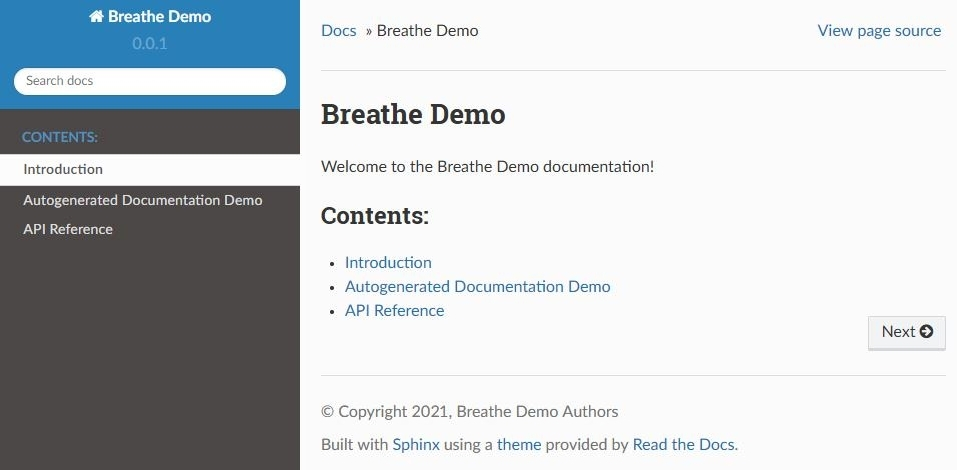
\includegraphics[width=0.9\textwidth]{content/1/chapter3/images/9.jpg}\\
Figure 3.9 – The main page of our documentation, consolidating both the generated and manually written parts
\end{center}

And when we look at the API docs page, it should look like this:

\begin{center}
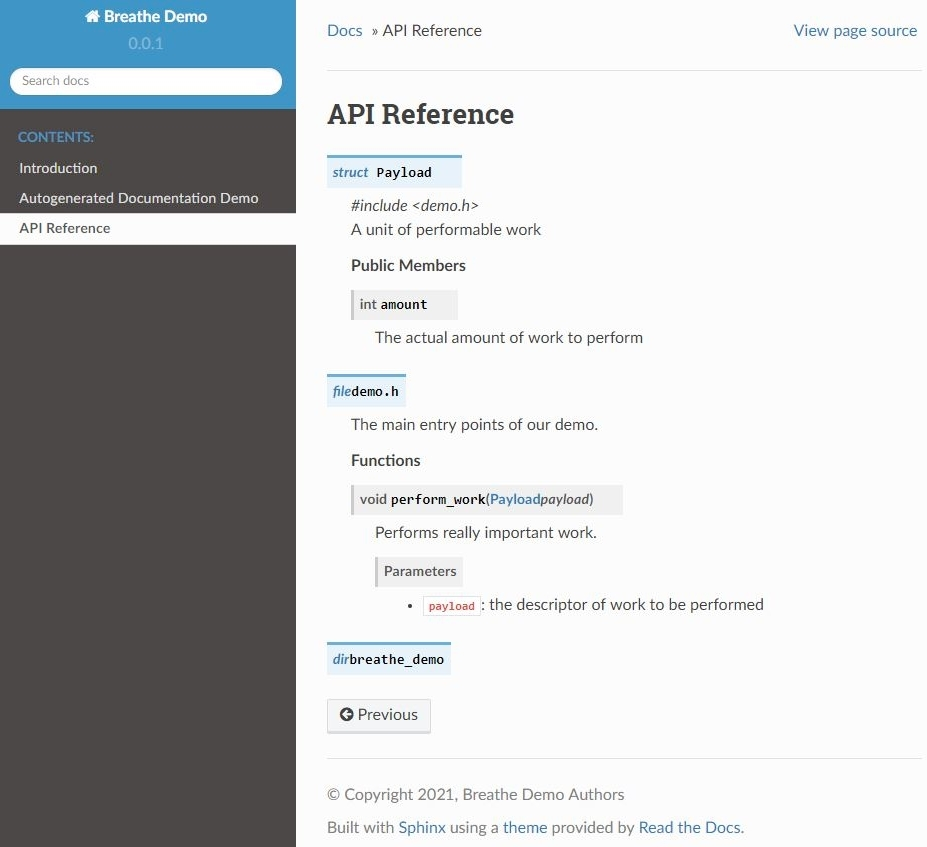
\includegraphics[width=0.9\textwidth]{content/1/chapter3/images/10.jpg}\\
Figure 3.10 – The automatically generated API documentation
\end{center}

As you can see, the documentation was automatically generated for our \textit{Payload} type with each of its members, as well as for the free \textit{perform\_work} function, including each of its parameters, and was grouped based on the file that defines them. Neat!

























